\documentclass[12pt,a4paper,onecolumn,titlepage]{report}
%when apply twoside next page moves to left
\usepackage{geometry}
\geometry{
	a4paper,
	left=35mm,
	right=25mm,
	top=25mm,
	bottom=25mm,
}
\usepackage[polish,english]{babel}
\usepackage[utf8]{inputenc}
\usepackage{ot1patch}
\usepackage[T1]{fontenc}
\usepackage{todonotes}
\usepackage{hyperref}
\usepackage{listings}
\usepackage{setspace}
\usepackage{times}
\usepackage[multiple]{footmisc}
\usepackage{mathtools}
\usepackage{amsfonts}
\usepackage{array,tabularx}
\usepackage{algorithm2e}
\lstset{frame=trBL}
\lstset{captionpos=b}
\lstset{numbers=left}
\lstset{breaklines=true}

\lstdefinestyle{BASH}{language=bash,frame=tb,numbers=left,numberstyle=\tiny,columns=fullflexible,
	backgroundcolor=\color{yellow!20},basicstyle=\small\sffamily, breaklines=true}

\lstdefinestyle{JAVA}{language=Java,numbers=left,numberstyle=\tiny,backgroundcolor=\color{yellow!20},basicstyle=\small\sffamily,breaklines=true,frame=tb}
%links are not coloured
\hypersetup{hidelinks}
\onehalfspacing

\newenvironment{conditions*}
{\par\vspace{\abovedisplayskip}\noindent
	\tabularx{\columnwidth}{>{$}l<{$} @{\ : } >{\raggedright\arraybackslash}X}}
{\endtabularx\par\vspace{\belowdisplayskip}}

\title {Bacherol Thesis
\\Points of Interests categorization system}
\author{Szymon Łyszkowski}

\begin{document}
\maketitle

\textbf{
		\\Faculty of Technical Physics, Information Technology and Applied \\Mathematics
		\\Thesis supervisor: Piotr Skulimowski, PhD
		\\Graduate student: Szymon Łyszkowski
		\\Index number: 171132
		\\Programme: Information Technology
	}


\tableofcontents

\chapter{Introduction} \label{chap.introduction} 
{Nowadays thanks to unlimited internet access we can gather enormously huge amount of data easily within rapid pace. The main problem which occurs is to simplify the access to the content which is expeced from user. People upload a lot of information not neccesserily mark with appropriate sign to find it again fast. Such problem lead to develop a system which would facilitate data organization. Especially categorization is expected in GIS\footnote{Geographic Information System} e.g. Web-based application enabling map visualization or PND\footnote{Portable Navigation Device}.

}


\section{Problem and Thesis Scope}
This thesis is describing complex problem of POI\footnote{Points of Interest} categorization and its possible solutions. Computer Information System which can facitlitate to solve given problem was implemented as a practical part. Document contains also description of methods which can be applied to categorize data (which in this case is plain text). 

\section{Thesis Objectives}
As main objective was to prepare ready to use java library which would enable user flexible API\footnote{Application Programmer Interface}. In this context word 'flexible' means that user can provide data in unstuctured form and obtain result as a category of given input. Such library can be imported as plain jar file without any additional sources as it is compiled with all dependencies. The only one requried source is input data which should be provided by user as a working material. 

\section{Research Method}
As mentioned before a categorization is complex problem which has to be customized according to given data. There are a lot of text processing methods to apply. Some of them were considered to be used e.g. preprocessing, feature extraction, train classifier, SVM\footnote{Support Vector Machine}, VSM\footnote{Vector Space Model}.

\section{Document Organization}
\todo{When done describe document ordering and organization (chapters)}
\chapter{Categorization Methods}
\section{Overview}
Plain text is the most friendly and convenient in use for human beings as a data medium. Unfortunately amount of text which can be effectively analyzed by human is quite limited. On the other hand, text as source of information for computer machines does not possess any heuristics. That is the reason to develop methods which can be applied to for particular data sources selected by human. As text content is usually complex methods are designed in such way that cover narrow categories of data sources. In general methods taken under consideration in this thesis were covering following approaches:
\begin{itemize}
	\item Preprocessing - text analysis paying special attention to reject unnecessary phrases which would slow down categorizarion process.
	\item Feature Extraction - text analysis which can consider wide range of text. Useful especially to analyze human text input (internet forum comment and entries). Uses TF-IDF\footnote{Term Frequency-Inverse Document Frequency} method.
	\item Naive Bayesian Classifier - method enabling direct text classification to appropriate category/phrase. It requires initial knowledge (heuristics) about given input.
	\item SVM\footnote{Support Vector Machine} - a form of binary classification. It divides input to two different separable domains. In order to classify for particular domain one-to-one comparison is applied.
	\item VSM \footnote{Vector Space Model} - method of text indexing and weight measuring. Already weighted indices are easier to give a hint for human which document to query. In the last stage measures text content simillarity according to given query.
	       
\end{itemize}

\section{Preprocessing}
The most important function of preprocessing is obviously downsizing of input data. Redunant or non-heuristic data can influence factors like:
\begin{itemize}
	\item Performance - the less text to analyze the result can be obtained faster
	\item Complexity - unnecessary phrases can influence in futher steps on classification correctness (dim heuristics)
	zawartość...
\end{itemize}

The most often rejected phrases are those which appear the most frequently in particular language. Concering english language phrases like: \textit{the, a, e.g, i.e} does not introduce any hint for further classification. This is the reason why processing of such statments can be abandoned in further steps. Each document should be human analyzed properly before applying patterns to reject. Patterns will differ significantly if given input will be database entry, HTML page or plain forum comment. 



 
\chapter{Loadstone SQLite Database}\label{chap.loadstone}

\section{Overview}
Problem of POI categorization comes for many data sources. One of them is database which is used in legacy Symbian applications which are used by blind people. Such applications are difficult to migrate fluently to newer platforms used in high-tech smartphones e.g iOS or Android. Such data are organized in difficult to analyze text files. Examplary database files can be found on Loadstone project website: \url{http://gps.zlotowicz.pl}. The purpose of this thesis was to prepare ready to use source data for Java-based platform Android. Such approach allows programmer to easily invoke java methods delivering source data in convenient way.

\section{SQLite Conversion}
To deliver easy access solution source *.txt files were converted to SQLite database. SQLite database gives opportunity to compress data effectively and are widely used in smartphones were resources need to have limited size. To build SQLite database special bash shell script had to be developed:

\begin{lstlisting}[style=BASH]	
#!/bin/sh
sqlite3 $2.db <<EOS
.headers on
CREATE TABLE LoadstoneTotalDataObjectModel (
"name" TEXT,
"latitude" REAL,
"longitude" REAL,
"accuracy" REAL,
"satellites" INTEGER,
"priority" INTEGER,
"userid" INTEGER,
"id" INTEGER
);
.separator ,
.import $1 TotalData
CREATE TABLE DatabaseInfo ( version INT, createdDate DATETIME, accessedDate DATETIME);
INSERT INTO DatabaseInfo(version, createdDate, accessedDate) VALUES (1,datetime('now'),datetime('now'));
.tables
.schema TotalData
.schema DatabaseInfo
EOS
\end{lstlisting}

As first input parameter of the script is path to .txt file which contains data supposed to be converted to SQLite database. As second parameter takes resultant database name. Invoke example in bash shell:
\begin{lstlisting}[style=BASH]
chmod +x createDB.sh #makes script executable
createDB.sh /directory/to/txt/file/cala_polska.txt dataBaseNameWithoutExtention
\end{lstlisting} 
\chapter{Categorization API}
As mentioned before main purpose of this thesis is POI classification. Unfortunately main topic is difficult to isolate because it involves custom input data. In previous chapter preparation and implementation of custom input data was described. This chapter will cover the topic of categorization data which are already delivered to the system.

\section{POI Categories}

\subsection{Overview}
To effectively categorize POI there has to be defined appropriate category hierarchy. There are a lot of multiple standards which are widely used in many different solutions and technologies. Unfortunately there is no world-wide standard defined for POI categories. More frequent observation can be done when looking at companies like: \textbf{Garmin, TomTom, Waze} that those entities try to introduce their own solutions. Garmin offers its own \textit{POILoader} which allows for own category definition \cite{9}. On the other hand TomTom offers 500 different POI categories by default \cite{10} but if user is eager to add custom POIs additional steps need to be done. User must prepare his own files with extension \textbf{\textit{.ov2}} and deploy it on GPS device. What is more deployment process depend on device model. Waze also defines it's own POI category standard \cite{14} There is an endeavour done by \textbf{W3C} organization about standarizing POI Data Model unfortundately according do W3C wiki it is still in beta version and categories definied is supposed to be defined in future \cite{12}. Only XML standard was defined (which supposed to be used as world-wide standart for POI data transfer) \cite{13}
\begin{figure}
	\centering
	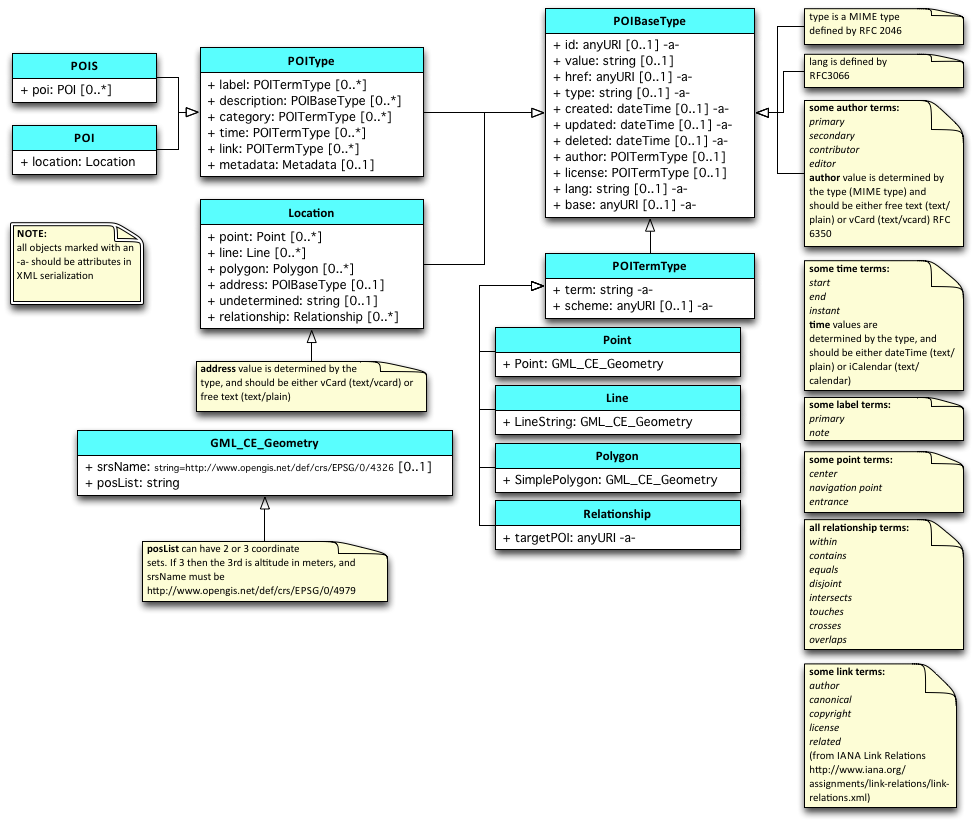
\includegraphics[scale=0.5]{W3c_poi_model.png}
	\caption{W3C UML Diagram POI Data Model}
	\label{fig:@=w3cDataModel}
\end{figure}
There is an apprehensible delamination in field of POI categories. It is difficult to find a standard which could be useful and well known for every data source. Fortunately there are standards defined by governments which describe categories in very detailed way and have endorsement by substantive position as countries governments possess. 
\subsection{NAICS}
\textit{\textbf{The North American Industry Classification System (NAICS)}} widely used in countries of North America. Developed by three organizations:  U.S. Economic Classification Policy Committee (ECPC), Statistics Canada, Mexico's Instituto Nacional de Estadistica y Geografia. It is mainly used by Federal agencies to collect data about bussiness entites for statistic purposes. It is successor of \textit{\textbf{Standard Industrial Classification (SIC)}}. NAICS classification is basing on codes which correspond to category description. Code can at most consist of six digits (the more digits included in code the more detailed category description is). Latest NAICS revision was issued in 2012. \cite{15} \cite{16}
\subsection{NACE}
\textit{\textbf{Statistical Classification of Economic Activities in the European Community (in French: Nomenclature statistique des activités économiques dans la Communauté européenne) - NACE}} system widely used in European Union. Similarly to NACE it is using combination of codes and category description. Code consists of letter and digits and creates special hierarchy of: sections, divisions, groups and classes. Section is marked by letter, division by two digits, groups and classes by one digit consecutively. Latest NACE revision (Rev.2) was issued in 2008 as a result of constantly developing and  newly appearing organizations especially in telecommunication business.\cite{17} \cite{18} Because java application which is purpose of this thesis was developed in Poland NACE categorization standard was chosen to apply in it. Obviously information included in NACE are definitely too much detailed to be applied for POI categorization system so only sections were taken into consideration. 

\section{Java library as categorization API}
\todo{cel api - zrodla danych, rezultat, metody processingu API = connection, classification, utilsy, czemu taki a nie inny podzial na pakiety - opis unit testow}
Main purpose of Java categorization API is to deliver an interface which would allow for convenient, correct and efficient results. API should be independent of data type which will be delivered. API responsibility is to enable functionalities (as this thesis states - categorization). To assure independence of data sources powerful mechanism of java interfaces can be used - such approach introduce level of abstraction and allow java library for easy communication with data sources. Java has very useful feature of importing and using libraries - when whole code is compiled to bytecode classes are bundled into resultant \textbf{\textit{.jar}} file - it can be immediately used in another java project by another programmer. Moreover, resultant java library project can be compiled with dependencies so programmer who will use library later will not have to bother about classes which were used during library development are were not part of Java API \cite{19}. This approach increases size of \textbf{\textit{.jar}} file but realease user from inconvenient dependencies downloading nad importing into project.    

\subsection{Packages organization}
API is divided into three packages: \textit{connection, classification} and \textit{utils}. Such packaging organization assures clear and concise representation of API functionalites and utilities. Functional packages are divided into simillar hierachy to interfaces and packages responsible for particular data source handling (see figure \ref{fig:@=packages_oragnization}). For purpose of this thesis these packages were named \textit{loadstone}. Obviously unit tests for corresponding executing classes are located into separate directory (according to maven directory structure \cite{20}) but are included in the same packages (for java it is counterpart of namespace).
\begin{figure}[h]
 	\centering
 	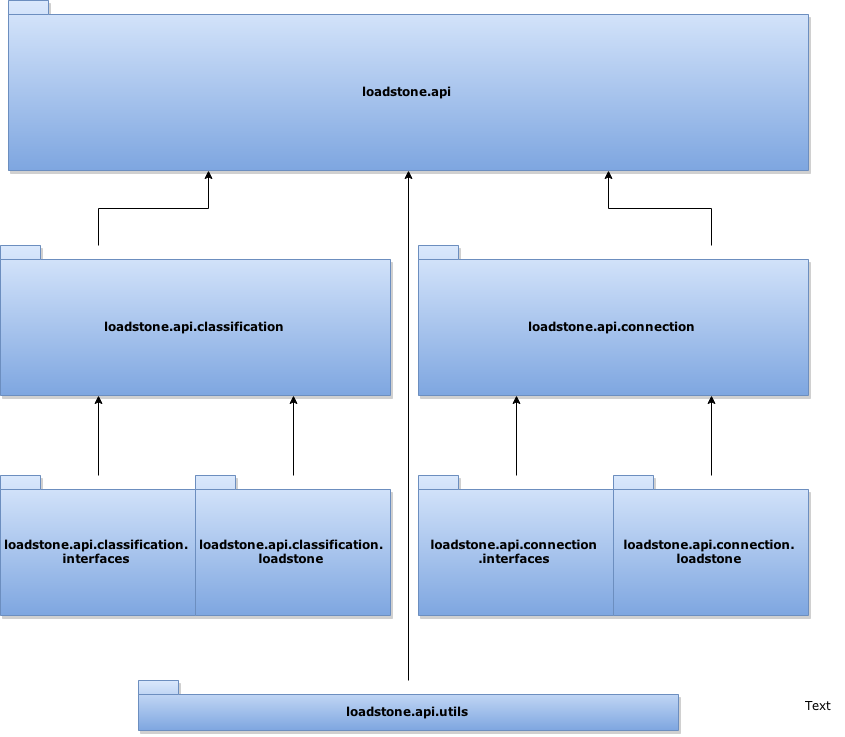
\includegraphics[scale=0.5]{loadstone_api_packages.png}
 	\caption{Loadstone API packages organization}
 	\label{fig:@=packages_oragnization}
\end{figure}
\subsection{Interface \newline loadstone.api.classification.interfaces.\newline AbstractResourcePreprocessing}
As mentioned before independence of input data is absolutely compulsory for API. To define preprocessing for each different kind of data source  AbstractResourcePreprocessing interface was defined. Classes which will be strictly delegated to preprocess particular source of data by implementation of this interface will be able to communicate with API and pass already preprocessed data for further classification methods.Interface also relies on model object data (DataModel) which is defined in another module of the project - \textbf{loadstone-model}. This assures for uniform and scalable solution for next data resources. AbstractResourcePreprocessing defines two methods which has to be implemented by data source dedicated classes to use categorization methods. Interface organization is depicted in the figure \ref{fig:@=AbstractResourcePreprocessing}:
\begin{figure}[h]
	\centering
	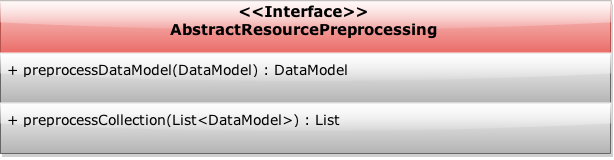
\includegraphics[scale=0.5]{AbstractResourcePreprocessing.png}
	\caption{AbstractResourcePreprocessing UML Diagram}
	\label{fig:@=AbstractResourcePreprocessing}
\end{figure}
\subsection{Interface \newline loadstone.api.classification.Classifier}
This interface is devoted for classes implementing classification functionalites. It imposes on classes to deliver data soure in appopriate way and return List. Main idea of this interface is to inform user that every data model object can be assigned to one or more classes. UML diagram on figure \ref{fig:@=classifier}
\begin{figure}[h]
	\centering
	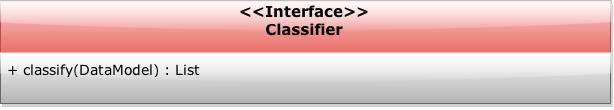
\includegraphics[scale=0.5]{classifier_interface.png}
	\caption{Interface Classifier UML Diagram}
	\label{fig:@=classifier}
\end{figure}
\subsection{Interface \newline loadstone.api.connection.interfaces.AbstractResourceConnection}
Interface to uniform the input point for data source to API. Each new data source should implement its own class for data gathering and return it in a way interface indicate it. Then data from any other resource (e.g. loadstone database, RESTful API) can be delivered for categorization functionalities. AbstractResourceConnection is simillar to AbstractResourcePreprocessing because of imposing data delivery in term of data model single object and its collection. Interface organization is depicted in the figure \ref{fig:@=connection}   
\begin{figure}[h]
	\centering
	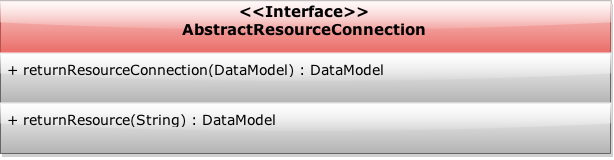
\includegraphics[scale=0.5]{Abstract_Resource_Connection_Interface.png}
	\caption{Interface AbstractResourceConnectionInterface UML Diagram}
	\label{fig:@=connection}
\end{figure}
Parameters for interface are respectively: List of Strings and String. Parameter types should be sufficient for particular data source invocation composition (e.g SQL statment). Using String type give user big flexibility if we are considering java as programming language.
\subsection{Class \newline loadstone.api.classification.loadstone.\newline LoadstonePreprocessing}
This class is deliberately delegated to preprocess data obtained from \textit{Loadstone} database. Using dedicated interface it assures final user about possibility of preprocesssing in easy to use and in the same time customized way. Class architecture is shown on \ref{fig:@=LoadstonePreprocessing}
\begin{figure}[h]
	\centering
	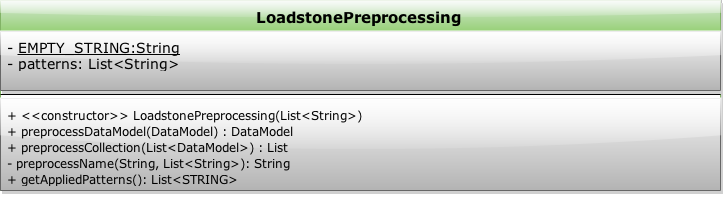
\includegraphics[scale=0.5]{LoadstonePreprocessing.png}
	\caption{LoadstonePreprocessing UML Diagram}
	\label{fig:@=LoadstonePreprocessing}
\end{figure}
Class organization is simple. For preprocessing functionality is responsible private method used in methods implementation of AbstractResourcePreprocessing interface. It simply process given input - rejects spaces (default behaviour) and patterns defined by user in constructor. Method is applied for single object DataModel or collection of such objects in corresponding interface methods.
\subsection{Class \newline loadstone.api.classification.loadstone.LoadstoneBOW}
\label{loadstone_bow}
This class is a feature for semi-supervised classification. It is basically a hashmap which values are sections of NACE categorization system and keys are strings which were the most frequenait occuring in loadstone database and assigned empirically to particular category. This class avails user to travers through map and check if category can be assigned immediately. 
\subsubsection{Bash script analyzeDB.sh}
\label{analyze_db}
Frequency for bag of words was prepared using bash shell script using awk tool which is great utility for text analysis \cite{21}. Script traverses through the loadstone database text file and counts occurrence of each word which exists in document. Algorithm can be expressed in following way:
\begin{algorithm}[h]
	\KwData{All words existing in loadstone database text file}
	\KwResult{Number of occurrences for each word}
	initalize array \textbf{words[]};
	\newline
	\ForEach{ \textit{word} in text file}
	{
		transform \textit{word} to lower case (avail disambiguation)
		\newline
		increase value by one for index \textit{word} in array \textbf{words[]} 
	}
	\ForEach{\textit{index-word} in \textbf{words[]}}{
		\Return word frequency:\textbf{words[\textit{index-word}]} for \textit{index-word} 	
	}
\caption{Analyzing frequency of words in database}\label{alg:analyze_freuency}
\end{algorithm}

Basing on Algorithm \ref{alg:analyze_freuency} it was possible to easily define those phrases which were most occuring and were significant or absolutely unncessary for text categorization. Obtaing list of words with their occurences in document there could be selected which can be used in BOW and which can be used for preprocessing as a hint.

\subsection{Class \newline loadstone.api.classification.NaiveClassifier}
\label{naive_classifier}
This class is implementing naive classification basing on descriptions from NACE\_Categories class using Classifier interface. It analyzes if data model name contains word which is included in particular category description. If data model name contains two or more words from distinct categories descriptions both of them are returned as possible categories to be assigned. This class is basing only on heuristic of NACE\_Categories descriptions so can be used for any data source but categorization correctness may differ significantly on data source.

\subsection{Class \newline loadstone.api.classification.loadstone.\newline LoadstoneSemiSupervisedClassifier}
Class which enables to classify POI using class LoadstoneBOW prepared previously. This class does not include descriptions from class NACE\_Categories. Only descriptions from LoadstoneBOW are taken into consideration. This class is implementing Classifier interface so it can be fluently used later in API.

\subsection{Class \newline loadstone.api.connection.loadstone.LoadstoneDatabase}
This class takes responsibility for gathering loadstone database. This class is implementing AbstractResourceConnection to get all possible entities from loadstone database. 
 
\subsubsection{LoadstoneDatabaseUpdater Singleton Design Pattern}
To modify data inside database loadstone.api.connection.loadstone.LoadstoneDatabaseUpdater should be used. It is using Singleton pattern to assure atomicity of operation on database. It defines static method \textit{getObjectModelSingleton()} returns static object on which user can work to modify data. Such approach allows for data correctness without bothering some other object is using database.  

\subsection{Class loadstone.api.utils.LoadstoneAPIUtils}
This class is just utility for user to construct appropriate SQL query to loadstone database. This utility only expect from user to input patterns which are supposed to be included during search for expected tuples in database. 

\subsection{Class loadstone.api.CategorizationAPI}
Class which can be enabled for final usage by user. It combines all methods of preprocessing, data source connection and classification methods. Should be used as input point for data considered to be classified and methods used for classification. Optionally user can add preprocessing method if step of this kind may be useful when POI classification is done.

\begin{figure}[h]
	\centering
	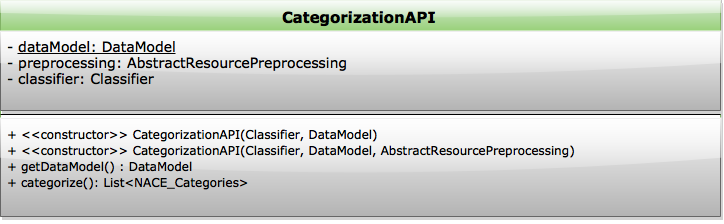
\includegraphics[scale=0.5]{CategorizationAPI.png}
	\caption{CategorizationAPI UML Diagram}
	\label{fig:@=CategorizationAPI}
\end{figure}
\chapter{Application Architecture}
\section{Overview}
This chapter describes application architecture which was purpose of this thesis. Application is organized into \textbf{four} essential parts:
\begin{itemize}
	\item Data source: loadstone DBMS
	\item Module 1: loadstone-model
	\item Module 2: loadstone-api
	\item Module 3: loadstone-package
\end{itemize}

\textit{Note: naming convention can differ from standard UML definitions. Module can be considered as component - represents a modular part of a system, that encapsulates its content and whose manifestation is replaceable within its environment. A component defines its behaviour in terms of provided and required interfaces \cite{22}. Module convention comes from the fact that application life-cycle and dependency management is marshalled by tool \textbf{Maven}. Maven uses naming convention of modules and helps developer to avoid introducing circular dependencies so application is easier to maintain in future} \cite{23}.

\section{Architecture scheme}
In the figure \ref{fig:@=architecture} is depicted overall architecture of Loadstone application.
\begin{figure}
	\centering
	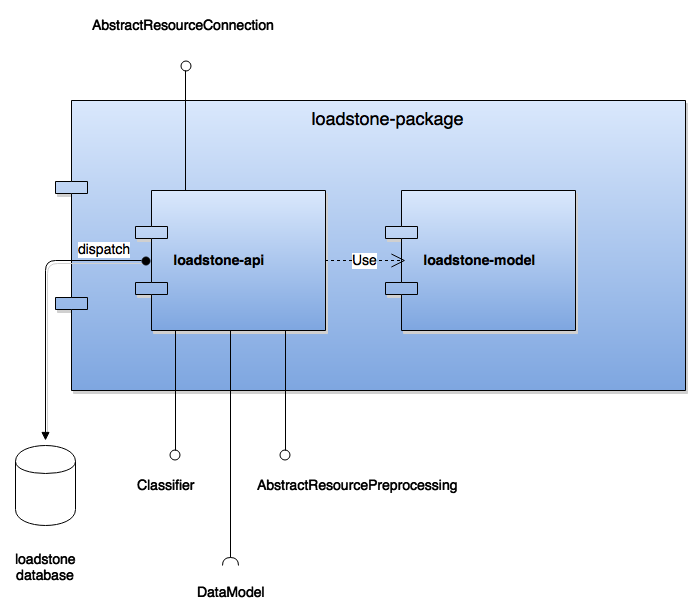
\includegraphics[scale=0.6]{architecture.png}
	\caption{Loadstone application architecture}
	\label{fig:@=architecture}
\end{figure}

\section{Architecture UML Class diagram}
To explore more implementation of application figure \ref{fig:@=loadstone_uml} should be analysed. It clearly describes technical details of application.
\begin{figure}
	\centering
	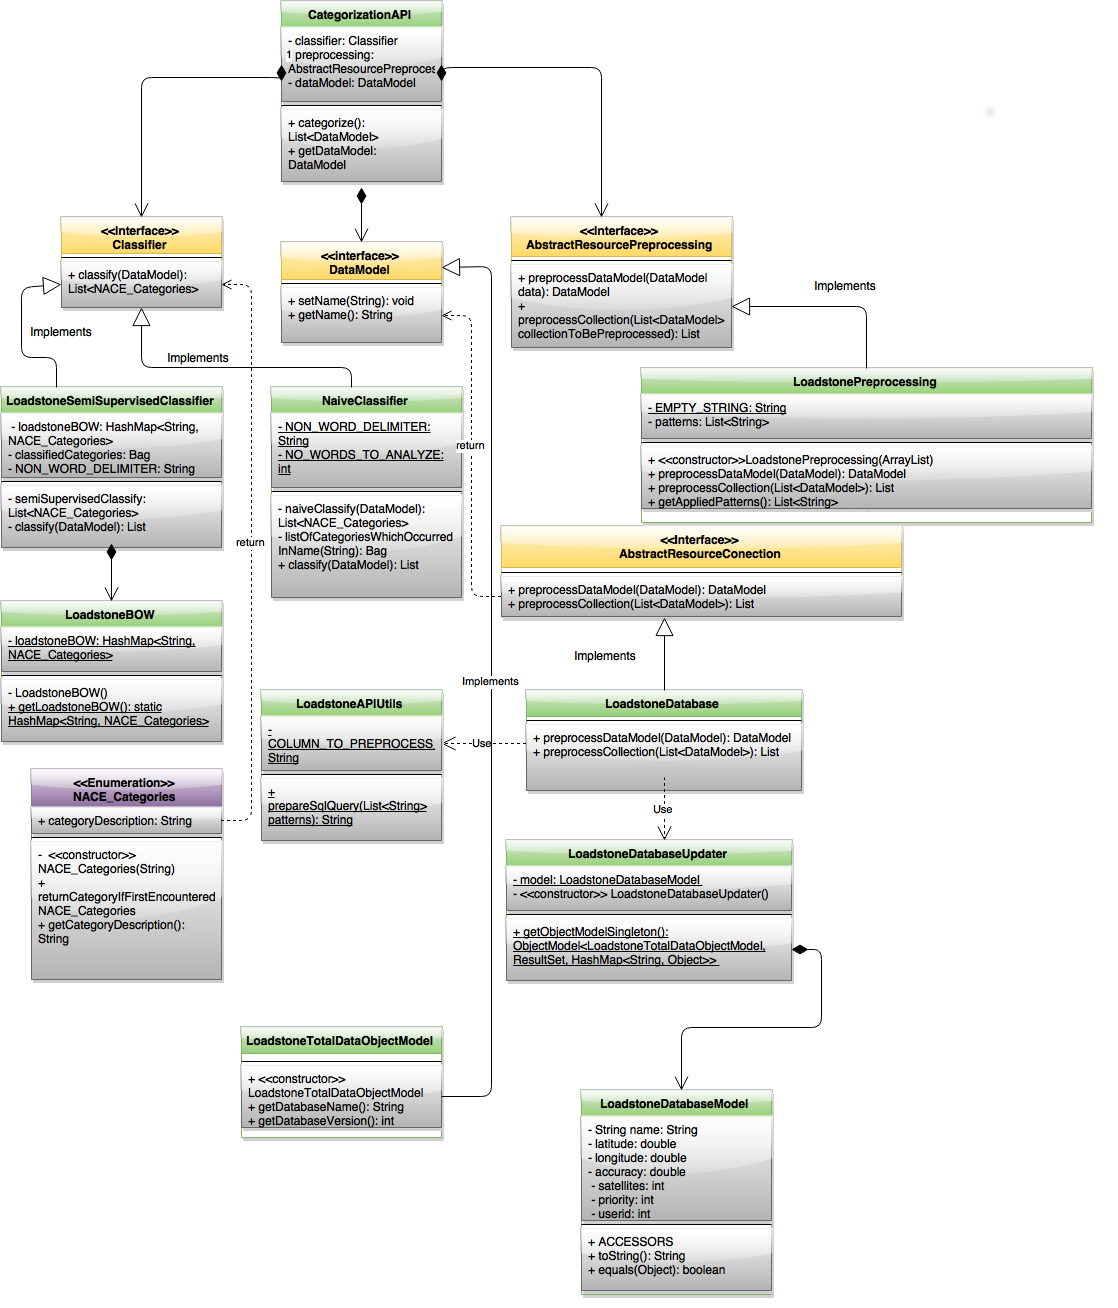
\includegraphics[scale=0.4]{UML.png}
	\caption{Loadstone application UML Class Diagram}
	\label{fig:@=loadstone_uml}
\end{figure}

\section{POI Categories}

\subsection{Tendency in POI categories}
To effectively categorize POI there has to be defined appropriate category hierarchy. There are a lot of multiple standards which are widely used in many different solutions and technologies. Unfortunately there is no world-wide standard defined for POI categories. More frequent observation can be done when looking at companies like: \textbf{Garmin, TomTom, Waze} that those entities try to introduce their own solutions. Garmin offers its own \textit{POILoader} which allows for own category definition \cite{9}. On the other hand TomTom offers 500 different POI categories by default but if user is eager to add custom POIs additional steps need to be done \cite{10}. User must prepare his own files with extension \textbf{\textit{.ov2}} and deploy it on GPS device. What is more deployment process depend on device model. Waze also defines it's own POI category standard \cite{14}. There is an endeavour done by \textbf{W3C} organization about POI Data Model standard (figure: \ref{fig:@=w3cDataModel}). Unfortunately according do W3C wiki it is still in beta version and categories are supposed to be defined in future \cite{12}. Only XML standard was developed (which supposed to be used as world-wide standard for POI data transfer) \cite{13}.
\begin{figure}[h]
	\centering
	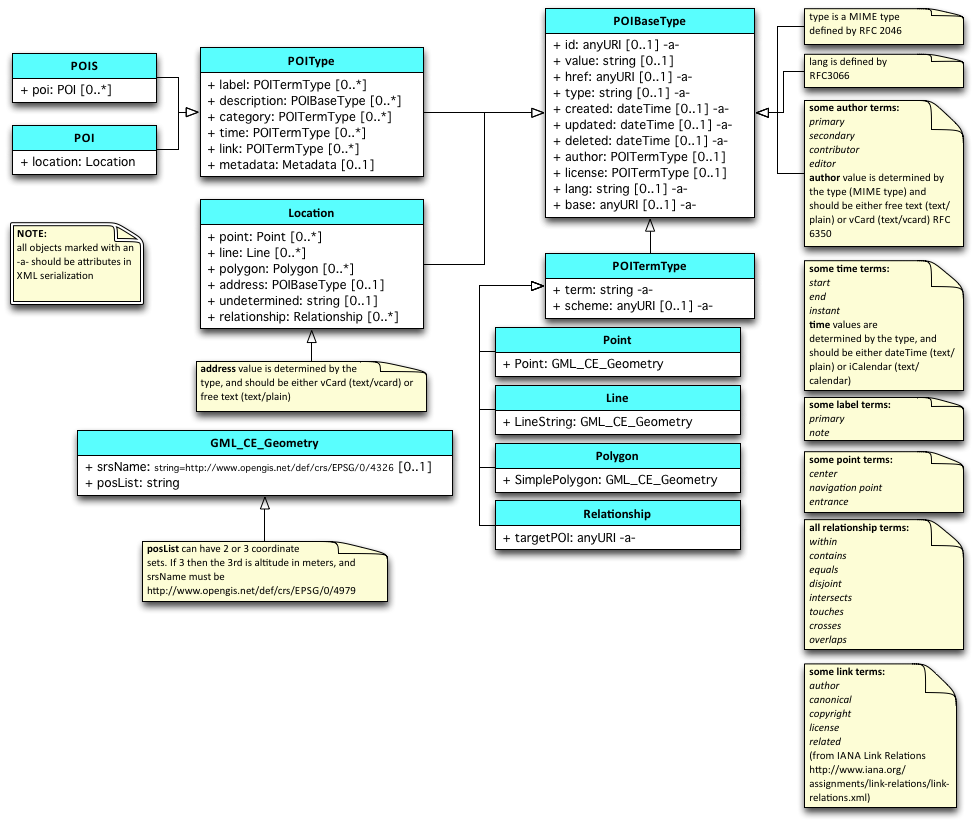
\includegraphics[scale=0.5]{W3c_poi_model.png}
	\caption{W3C UML Diagram POI Data Model}
	\label{fig:@=w3cDataModel}
\end{figure}
There is an apprehensible delamination in field of POI categories. It is difficult to find a standard which could be useful and well known for every data source. Fortunately there are standards defined by governments which describe categories in very detailed way and have endorsement by substantive position as countries governments possess. 
\subsection{NAICS}
\textit{\textbf{The North American Industry Classification System (NAICS)}} widely used in countries of North America. Developed by three organizations:  U.S. Economic Classification Policy Committee (ECPC), Statistics Canada, Mexico's Instituto Nacional de Estadistica y Geografia. It is mainly used by Federal agencies to collect data about business entities for statistic purposes. It is successor of \textit{\textbf{Standard Industrial Classification (SIC)}}. NAICS classification is basing on codes which correspond to category description. Code can at most consist of six digits (the more digits included in code the more detailed category description is). Latest NAICS revision was issued in 2012 \cite{15} \cite{16}.
\subsection{NACE}
\label{NACE}
\textit{\textbf{Statistical Classification of Economic Activities in the European Community (in French: Nomenclature statistique des activités économiques dans la Communauté européenne) - NACE}} system widely used in European Union. Similarly to NACE it is using combination of codes and category description. Code consists of letter and digits and creates special hierarchy of: sections, divisions, groups and classes. Section is marked by letter, division by two digits, groups and classes by one digit consecutively. Latest NACE revision (Rev.2) was issued in 2008 as a result of constantly developing and  newly appearing organizations especially in telecommunication business \cite{17} \cite{18}. Because Java application which is purpose of this thesis was developed in Poland NACE categorization standard was chosen to apply in it. Obviously information included in NACE are definitely too much detailed to be applied for POI categorization system so only main sections were taken into consideration \cite{31}. Assignment of category and description is presented in table \ref{tab:NaceMatching}.
\begin{table}[H] 
	\begin{tabular}{ | c | c |}
		\hline
		Category & Description\tabularnewline \hline
		A & Agriculture, forestry and fishing\\\hline
		B & Mining and quarrying\\\hline
		C & Manufacturing\\\hline
		D & Electricity, gas, steam and air conditioning supply\\\hline
		E & Water supply, sewerage, waste management and remediation activities\\\hline
		F & Construction\\\hline
		G & Wholesale and retail trade, repair of motor vehicles and motorcycles\\\hline
		H & Transporting and storage\\\hline
		I & Accommodation and food service activities\\\hline
		J & Information and communication\\\hline
		K & Financial and insurance activities\\\hline
		L & Real estate activities\\\hline
		M & Professional, scientific and technical activities\\\hline
		N & Administrative and support service activities\\\hline
		O & Public administration and defence, compulsory social security\\\hline
		P & Education\\\hline
		Q & Human health and social work activities\\\hline
		R & Arts, entertainment and recreation\\\hline
		S & Other services activities\\\hline
		T & \begin{tabular}{@{}c@{}}Activities of households as employers undifferentiated goods and services\\ - producing activities of households for own use\end{tabular}\\\hline
		U & Activities of extraterritorial organisations and bodies\\\hline
		NOT\_CLASSIFIED & Not classified\\ 		
		\hline
	\end{tabular}
	\caption{Implemented NACE categories with assigned human readable description}
	\label{tab:NaceMatching}
\end{table} 

\section{Java library as categorization API}
Main purpose of Java categorization API is to deliver an interface which would allow for convenient, correct and efficient results. API should be independent of data type which will be delivered. API responsibility is to enable functionalities (as this thesis states - categorization). To assure independence of data sources powerful mechanism of Java interfaces can be used - such approach introduce level of abstraction and allow Java library for easy communication with data sources. Java has very useful feature of importing and using libraries - when whole code is compiled to bytecode classes are bundled into resultant \textbf{\textit{.jar}} file - it can be immediately used in another Java project by another programmer. Moreover, resultant Java library project can be compiled with dependencies so programmer who will use library later will not have to bother about classes which were used during library development are were not part of Java API \cite{19}. This approach increases size of \textbf{\textit{.jar}} file but release user from inconvenient dependencies downloading and importing into project.    

\subsection{Packages organization}
API is divided into three packages: \textit{connection, classification} and \textit{utils}. Such packaging organization assures clear and concise representation of API functionalites and utilities. Functional packages are divided into similar hierarchy to interfaces and packages responsible for particular data source handling (figure \ref{fig:@=packages_oragnization}). For purpose of this thesis these packages were named \textit{Loadstone}. Obviously unit tests for corresponding executing classes are located into separate directory (according to maven directory structure) but are included in the same packages (for Java it is counterpart of namespace) \cite{20}.
\begin{figure}[h]
	\centering
	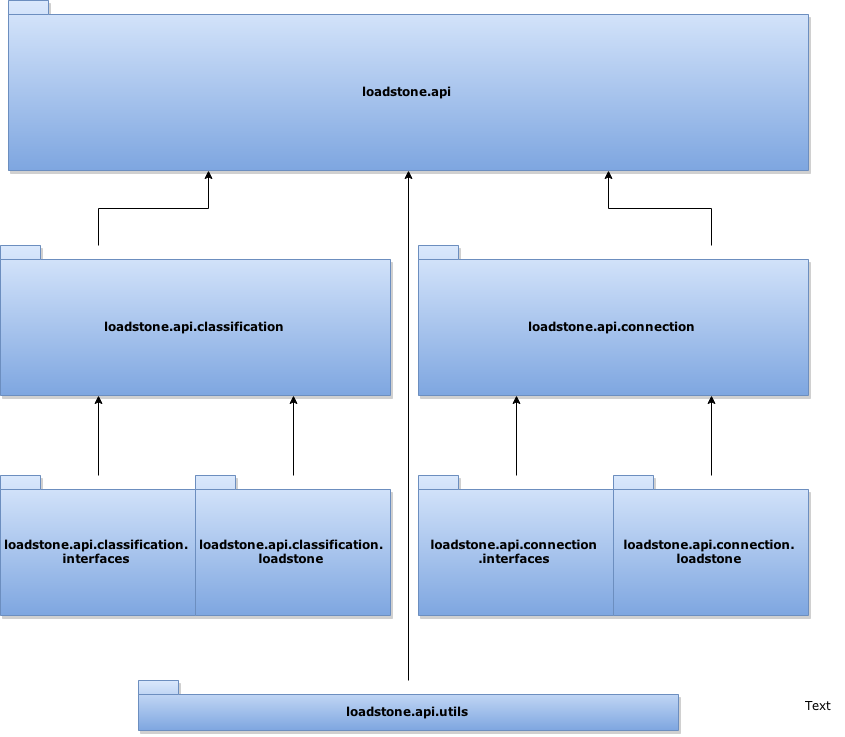
\includegraphics[scale=0.5]{loadstone_api_packages.png}
	\caption{Loadstone API packages organization}
	\label{fig:@=packages_oragnization}
\end{figure}
\subsection{Interface \newline loadstone.api.classification.interfaces.\newline AbstractResourcePreprocessing}
As mentioned before independence of input data is absolutely compulsory for API. To define preprocessing for each different kind of data source  AbstractResourcePreprocessing interface was defined. Classes which will be strictly delegated to pre-process particular source of data by implementation of this interface will be able to communicate with API and pass already preprocessed data for further classification methods.Interface also relies on model object data (DataModel) which is defined in another module of the project - \textbf{loadstone-model}. This assures for uniform and scalable solution for next data resources. AbstractResourcePreprocessing defines two methods which has to be implemented by data source dedicated classes to use categorization methods. Interface organization is depicted in the figure \ref{fig:@=AbstractResourcePreprocessing}:
\begin{figure}[h]
	\centering
	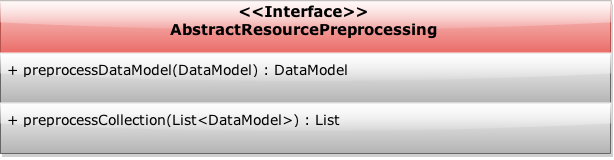
\includegraphics[scale=0.5]{AbstractResourcePreprocessing.png}
	\caption{AbstractResourcePreprocessing UML Diagram}
	\label{fig:@=AbstractResourcePreprocessing}
\end{figure}
\subsection{Interface \newline loadstone.api.classification.Classifier}
This interface is devoted for classes implementing classification functionalities. It imposes on classes to deliver data source in appropriate way and return List. Main idea of this interface is to inform user that every data model object can be assigned to one or more classes. UML diagram on figure \ref{fig:@=classifier}.
\begin{figure}[h]
	\centering
	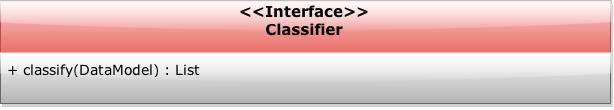
\includegraphics[scale=0.5]{classifier_interface.png}
	\caption{Interface Classifier UML Diagram}
	\label{fig:@=classifier}
\end{figure}
\subsection{Interface \newline loadstone.api.connection.interfaces.AbstractResourceConnection}
Interface to uniform the input point for data source to API. Each new data source should implement its own class for data gathering and return it in a way interface indicate it. Then data from any other resource (e.g. Loadstone database, RESTful API) can be delivered for categorization functionalities. AbstractResourceConnection is similar to AbstractResourcePreprocessing because of imposing data delivery in term of data model single object and its collection. Interface organization is depicted in the figure \ref{fig:@=connection}.   
\begin{figure}[h]
	\centering
	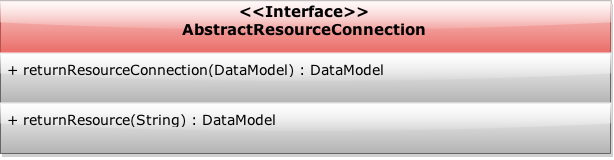
\includegraphics[scale=0.5]{Abstract_Resource_Connection_Interface.png}
	\caption{Interface AbstractResourceConnectionInterface UML Diagram}
	\label{fig:@=connection}
\end{figure}
Parameters for interface are respectively: List of Strings and String. Parameter types should be sufficient for particular data source invocation composition (e.g SQL statement). Using String type give user big flexibility if we are considering Java as programming language.
\subsection{Class \newline loadstone.api.classification.loadstone.\newline LoadstonePreprocessing}
This class is deliberately delegated to pre-process data obtained from \textit{Loadstone} database. Using dedicated interface it assures final user about possibility of preprocessing in easy to use and in the same time customized way. Class architecture is shown on \ref{fig:@=LoadstonePreprocessing}.
\begin{figure}[h]
	\centering
	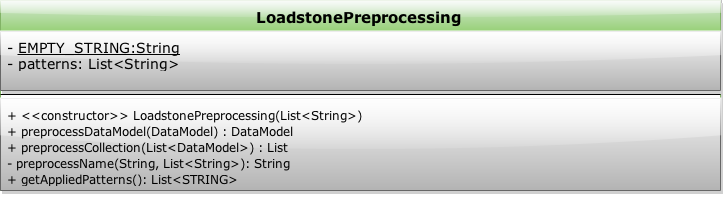
\includegraphics[scale=0.5]{LoadstonePreprocessing.png}
	\caption{LoadstonePreprocessing UML Diagram}
	\label{fig:@=LoadstonePreprocessing}
\end{figure}
Class organization is simple. For preprocessing functionality is responsible private method used in methods implementation of AbstractResourcePreprocessing interface. It simply process given input - rejects spaces (default behaviour) and patterns defined by user in constructor. Method is applied for single object DataModel or collection of such objects in corresponding interface methods.
\subsection{Class \newline loadstone.api.classification.loadstone.LoadstoneBOW}
\label{loadstone_bow}
This class is a feature for semi-supervised classification. It is basically a hashmap which values are sections of NACE categorization system and keys are strings which were the most frequent occurring in Loadstone database and assigned empirically to particular category. This class avails user traversing through map and check if category can be assigned immediately. Empirically assigned categories to BOW are presented in table: \ref{tab:BowMatching} \textbf{(it is sample of implementation)}.
\begin{table}
	\centering 
	\begin{tabular}{ | c | c |}
		\hline   
		Category  & BOW member\tabularnewline \hline
		bankomat  & K\\\hline
		kościół & U\\\hline
		kurier&J\\\hline
		pgp & J\\\hline
		szkoła & P\\\hline
		atm & K\\\hline
		cmentarz & U\\\hline
		supermarket & G\\\hline
		apteka & Q\\\hline
		bank & K\\\hline
		krzyż & U\\\hline
		most & H\\\hline
		spożywczy & I\\\hline
		restauracja & I\\\hline
		sklep & G\\\hline
		plac & H\\\hline
		hotel & I\\\hline
		euronet & K\\\hline
		bunkier & R\\\hline
		pomnik & R\\\hline
		jezioro & A\\\hline
		poczta & J\\\hline
		rynek & A\\\hline
		jedzenie & I\\\hline
		katolicki & U\\\hline
		pko & K\\\hline
		samochodowy & G\\\hline
		warsztat & G\\\hline
		szlak & A\\\hline
		biedronka & G\\\hline
		orlen & D\\\hline
		lpg & D\\\hline
		straż & O\\\hline
		myjnia & T\\\hline
	\end{tabular}
	\caption{BOW for loadstone database keywords assignments to categories}
	\label{tab:BowMatching}
\end{table} 

\subsection{Class \newline loadstone.api.classification.NaiveClassifier}
\label{naive_classifier}
This class is implementing naive classification basing on descriptions from NACE categories class using Classifier interface. It analyses if data model name contains word which is included in particular category description. If data model name contains two or more words from distinct categories descriptions both of them are returned as possible categories to be assigned. This class is basing only on heuristic of NACE categories section: \ref{NACE} descriptions so can be used for any data source but categorization correctness may differ significantly on data source.

\subsection{Class \newline loadstone.api.classification.loadstone.\newline LoadstoneSemiSupervisedClassifier}
Class which enables to classify POI using class LoadstoneBOW prepared previously. This class does not include descriptions from class NACE\_Categories. Only descriptions from LoadstoneBOW are taken into consideration. This class is implementing Classifier interface so it can be fluently used later in API.

\subsection{Class \newline loadstone.api.connection.loadstone.LoadstoneDatabase}
This class takes responsibility for gathering Loadstone database. This class is implementing AbstractResourceConnection to get all possible entities from Loadstone database. 

\subsubsection{LoadstoneDatabaseUpdater Singleton Design Pattern}
To modify data inside database loadstone.api.connection.loadstone.LoadstoneDatabaseUpdater should be used. It is using Singleton pattern to assure atomicity of operation on database. It defines static method \textit{getObjectModelSingleton()} returns static object on which user can work to modify data. Such approach allows for data correctness without bothering some other object is using database.  

\subsection{Class loadstone.api.utils.LoadstoneAPIUtils}
This class is just utility for user to construct appropriate SQL query to Loadstone database. This utility only expect from user to input patterns which are supposed to be included during search for expected tuples in database. 

\subsection{Class loadstone.api.CategorizationAPI}
Class which can be enabled for final usage by user. It combines all methods of preprocessing, data source connection and classification methods. Should be used as input point for data considered to be classified and methods used for classification. Optionally user can add preprocessing method if step of this kind may be useful when POI classification is done. UML diagram on figure \ref{fig:@=CategorizationAPI}

\begin{figure}[h]
	\centering
	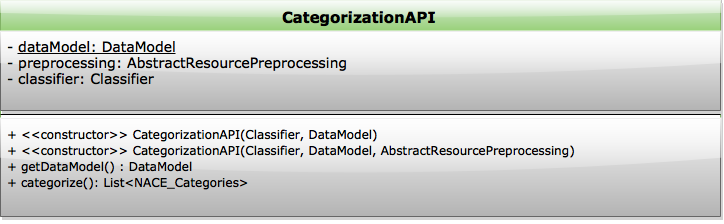
\includegraphics[scale=0.5]{CategorizationAPI.png}
	\caption{CategorizationAPI UML Diagram}
	\label{fig:@=CategorizationAPI}
\end{figure}

\section{Library Usage}
Product of created information system is API which can be used by programmer. Usage of library is simple and intuitive. Access to data source and semi-supervised classification task can be done in couple of lines in Java code. The following code snippet demonstrates how to execute categorization task using Loadstone database as data source. Chosen source data is first selected entry given by SQL query to database, contains phrase \textit{bankomat} and will be preprocessed from phrases: \textit{"ul.","adres" and "."}
\begin{lstlisting}[style=JAVA]
//define query condition
patternsToLookForInLoadstoneDatabase = new ArrayList<>();
patternsToLookForInLoadstoneDatabase.add("bankomat");
//patterns preparation for preprocessing
patternsToBeTrimmedFromConsideredDataModel = new ArrayList();
patternsToBeTrimmedFromConsideredDataModel.add("ul.");
patternsToBeTrimmedFromConsideredDataModel.add("adres");
patternsToBeTrimmedFromConsideredDataModel.add("\\.");
//Return data from database
List<DataModel> dataModels = new LoadstoneDatabase().returnResourceCollection(patternsToLookForInLoadstoneDatabase);
//takes first database entry satisfying query condition
dataModelConsidered = dataModels.get(0);
//Initial conditions for API - classification method, data source, preprocessing conditions
CategorizationAPI categorizationAPI = new CategorizationAPI(new LoadstoneSemiSupervisedClassifier(), dataModelConsidered,
new LoadstonePreprocessing(patternsToBeTrimmedFromConsideredDataModel));
//Execute categorization
List<NACE_Categories> nace_categories = categorizationAPI.categorize();
\end{lstlisting}
\chapter{Thesis results}

\section{Overview}
The main purpose of this thesis is to obtain categorization system for POIs. Such task is complex and difficult to execute for complex data which are present in modern word. It is very difficult to obtain desired results for each kind of data. Text processing is wide domain and requires a lot of computing power and time to return results which are readable for human. When some heuristics is applied processing effort can be decreased in both fileds of execution time and required computing power. As mentioned in previous chapters there are many methods which enable method categorization. What is more every method is aimed for different kind of input data. This can indicate that initial knowledge about input data is absolutely compulsory to achieve desired effect and effectiveness. In this chapter the results obtained from implemented information system will be presented for delivered source of data which is loadstone database.

\section{Preprocessing results}
Preprocessing is a task which does not involve high level of complexity in text analysis. It is very important to consider all combinations of \textit{\textbf{field separators}}(this therm denotes sign of space between analyzed words). Usually it is \textit{space} sign but not always. As already mentioned this may vary among input data and such signs could be \textit{tab key} or \textit{\_} sign. The best idea to apply text preprocessing is to collect statistics which would give information which phrases could be easily applied on data without any regression and conflicts on results. In case of loadstone database special bash script was prepared which is described in chapter section: \ref{analyze_db}. Results of this script gave heuristics which could be applied for preprocessing.
Phrases which can be rejected from analyzed text without any bothering about categorization corectness are as follows:
\newline
\begin{itemize}
	\item \textbf{\textit{"ul"}}
	\item \textbf{\textit{"adres"}}
	\item \textbf{\textit{"."}}
\end{itemize}
There is a test suite in \textit{loadstone.api.classification.loadstone.LoadstonePreprocessingTest} class which presents execution of preprocessing on specially prepared DataModel's for this purpose. Results for analyzed texts with those paricular patterns to be rejected from input text are as follows:

\begin{algorithm}
	\KwData{\textit{\textbf{"adres ul ul. fake name to be trimmed "}}}
	\KwResult{\textit{\textbf{"fake name to be trimmed"}}}
	\hfill \break
	\caption{Preprocessing example using mocked data}\label{alg:1st}
\end{algorithm}
This example shows that phrases: \textit{"adres ul ul. " and " "} were succefully rejected and there is significantly less data to analyze in further categorization process.
\newline
Another example is taken directly from loadstone database. Preprocessed text is an loadstone database entry.
\begin{algorithm}
	\KwData{\textit{\textbf{"adres ul. kramarska 15 warszawa rembertów"}}}
	\KwResult{\textit{\textbf{"kramarska 15 warszawa rembertów"}}}
	\hfill \break
	\caption{Preprocessing example using data extracted from loadstone database}\label{alg:2nd}
\end{algorithm}
\newline
As it is noticable also in this case preprocessing was successfull and did not rejected any data important from categorization point of view. Phrase: \textit{"adres ul. "} was trimmed correctly.
 
  
\section{Classification results}
\label{classification_results}
\subsection{Overview}
Classification is much more complicated task than preprocessing. It involves complex analysis of input data, possible misconceptions or inprecise heuristics. Moreover, categorization usually should be unambiguous but not always. Sometimes POI can be classified to more than one category as an example there can be considered a \textit{\textbf{church}} which can be categorized as \textit{"U - Activities of extraterritorial organisations and bodies "}(according to NACE standard notation) or may as well classified as \textit{"R - Arts, entertainment and recreation "}. However what is worth to mention is correlation between those two categories. POI \textit{\textbf{church}} cannot always be classified as the latter but always as the first one. Such cases can be complex and perfect solution is unlikely to find as well. The correctness of classification results may also vary among judging human beings.    
\subsection{Naive classifier categorization results}
As mentioned in chapter section: \ref{naive_classifier} naive classification bases on heuristics inherited from NACE standard. As heuristic for unambiguous results it takes information about frequency of given phrase in NACE category description. When one heuristic overcome in frequency second heuristic the latter is rejected. Two of more categories as result are returned when frequency is the same for each of given heuristic. When heuristic is not available in input data classification is unavailable. The following example can be presented for imaginary data:
\begin{algorithm}
	\KwData{\textit{\textbf{"Manufacturing Manufacturing Manufacturing Manufacturing Manufacturing Manufacturing administration administration administration"}}}
	\KwResult{\textit{\textbf{"C - Manufacturing "}}}
	\hfill \break
	\caption{Naive classifier example using mocked data for different phrase frequency}\label{alg:3rd}
\end{algorithm}
\newline
As heuristic \textbf{\textit{"Manufacturing"}} frequency was higher than \textbf{\textit{"administration"}} (six occurences versus three occurences) category C is returned as result for categorization system.
\newline
Another example demonstrate naive classification when heuristic frequency has the same value of occurences for each component:
\begin{algorithm}
	\KwData{\textit{\textbf{"Manufacturing Manufacturing Manufacturing administration administration administration"}}}
	\KwResult{\textit{\textbf{"C - Manufacturing ", "O - Public administration and defence; compulsory social security "}}}
	\hfill \break
	\caption{Naive classifier example using mocked data for uniform phrase frequency}\label{alg:4th}
\end{algorithm}
\newline  
As heuristic \textbf{\textit{"Manufacturing"}} frequency was the same as heuristic \textbf{\textit{"administration"}} category C and O is returned as result for categorization system.

\subsubsection{Naive classifier for loadstone database}

As heuristic is suit to data which are definitely not included in loadstone database input data description (main issue comparison between english and polish language) naive classifier does not have significant utility during loadstone database analysis. Algorithm \ref{alg:6th} proves it:
\begin{algorithm}
	\KwData{\textit{\textbf{"bankomat i oddział bz bwk atm 24h bank ul. jana pawła ii 12 sieradz"}}}
	\KwResult{\textit{\textbf{"Not classified"}}}
	\hfill \break
	\caption{Naive classifier using data extracted from loadstone database}\label{alg:5th}
\end{algorithm}
\newline  
As none heuristic exists in input data from NACE categories description "Not classified" result is returned.
\newline
\textit{Note: all examples are implemented as test suite of unit tests in class\newline loadstone.api.classification.NaiveClassifierTest}    
\subsection{Semisupervised categorization for loadstone database results}
Semisupervised categorization is very useful but requires much more complex analysis. It requires knowledge about heuristics included in input data. To perform semisupervised categorization loadstone bag of words was prepared previously (description chapter section: \ref{loadstone_bow}). Thanks to initial knowledge what kind of phrases could be used for categorization, results correctness is decent. Important factor is complete isolation from heuristics included in NACE standard category description (such apporach could possibly introduce regression) Following examples demonstrates performance of semisupervised categorization intended deliberately for input data derived from loadstone database:
\newline
\begin{algorithm}[h]
	\KwData{\textit{\textbf{"bankomat i oddział bz bwk atm 24h bank ul. jana pawła ii 12 sieradz"}}}
	\KwResult{\textit{\textbf{"K - Financial and insurance activities "}}}
	\hfill \break
	\caption{Semisupervised categorization using data extracted from loadstone database}\label{alg:6th}
\end{algorithm}
\newline
Because of heuristics: \textbf{\textit{bankomat, atm, bank}} which are defined in loadstone BOW are all assigned to category K unamigious result is retreived. This sample cleary demonstartes difference between naive (algorithm: \ref{alg:5th}) and semisupervised classification.
\newline
\begin{algorithm}[h]
	\KwData{\textit{\textbf{"bankomat and pizza"}}}
	\KwResult{\textit{\textbf{"I - Accommodation and food service activities ", "K - Financial and insurance activities "}}}
	\hfill \break
	\caption{Semisupervised categorization using mocked data with uniform phrase frequency}\label{alg:7th}
\end{algorithm}
\newline
Because of heuristics: \textbf{\textit{bankomat, pizza}} which are defined in loadstone BOW but are assigned to different categories the result is ambiguous. Heuristics frequencies are equal so two categories are returned as categorization results.
\newline
There was also performed comparision of imaginary data indicated deliberately to NACE standard category description analyzed by using method of semisupervised categorization. The result is as follows:
\begin{algorithm}[h]
	\KwData{\textit{\textbf{"Manufacturing Manufacturing Manufacturing Manufacturing Manufacturing Manufacturing administration administration administration"}}}
	\KwResult{\textit{\textbf{"Not classified"}}}
	\hfill \break
	\caption{Semisupervised categorization using mocked data not related to loadstoneBOW}\label{alg:8th}
\end{algorithm}
\newline
In comparison to algorithm \ref{alg:3rd} obtained result is completely irrelevant to reality and does not give correct result.
\newline 
\textit{Note: all examples are implemented as test suite of unit tests in class \newline loadstone.api.classification.LoadstoneSemiSupervisedClassifierTest}

\section{Conclusion}
The purpose of this thesis was to provide overview of categorization methods using text analysis which can be useful during POI classification. As a result of this research there was developed loadstone database (using script \textit{createDB.sh}) java library which delivers interface for \textit{loadstone} database access and provides categorization methods mainly suit for data included in database. Such customization was possible thanks to automatic analysis of phrase frequencies in database which functionality enables script \textit{analyzeDB.sh}. Library can be useful when developing applications using GPS systems to deliver information about POI in the neighbourhood. Main benefit of library is independence on data source so using specially designed interface there is possibility to delived many kind of data sources and combine it one application. The topic of POI categorization is wide and complex domain. This domain mainly involves text processing and heuristics about possible hints which can be used to obtain expected results. As presented in chapter section \ref{classification_results} result may differ according to applied categorization method. A lot of factors need to be considered when categorization task is applied like: language of input data, model of input data (it is possible to analyze whole documents or large fragment of texts or ready to use databases), size of input data (performance in complex infromation systems is one of significant factor). It is really difficult challange to estimate what kind heuristics data can be obtained and work out system which would be versatile for every data source. Another important factor is choice of technology for such information system. Java possess high native library support and community as well \cite{24} \cite{25}. Unfortunately this involves a lot of reasearch in internet to find suitable collection which can be used in implementation. What is more it is often practice that code construction is getting more complex and difficult to maintain in future. Example of such practice is returning classification result as \textit{list of categories} instead of using construction called \textit{tuple}. Such constructions are available in programming languages like: \textbf{Scala} \cite{26} or \textbf{Python} \cite{27}. What is more syntax of those programming languages is easier to read (it is possible to ommit longline java syntax - not so huge effort is pushed on object encapsulation) and flexibility. Another important issue are external tools which could be used for easier maintenance of infromation system. Such tool could be \textit{Apache Spark} \cite{28}. It increases the perfromance of execution and is great manager for feature extraction, transformations or SVM. On the other hand this technology is quite new and requires significant effort at the beginning to use it.     

\addcontentsline{toc}{chapter}{Bibliography}
\bibliography{sources}{}
\bibliographystyle{alpha}

\end{document}
